\begin{exercise}
      {ID-334183e3e3a655e89a6f9941dad85cf71fa9f60a}
      {Flächeninhalte}
  \ifproblem\problem
    Die in der Abbildung dargestellte Figur zeigt ein Rechteck $ABCD$ aus drei
    gleichgroßen Quadraten $AEHD$, $EFGH$ und $FBCG$. Die Kanten der Quadrate
    sind jeweils \sicm{6} lang.
    \begin{center}
      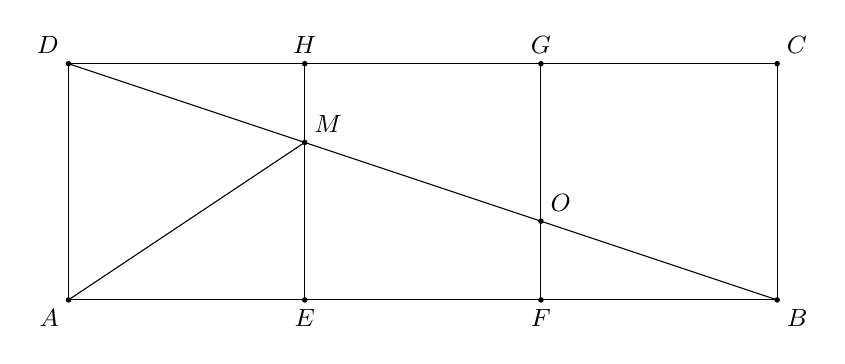
\begin{tikzpicture}
        \coordinate (A) at (0, 0);
        \coordinate (B) at (9, 0);
        \coordinate (C) at (9, 3);
        \coordinate (D) at (0, 3);
        \coordinate (E) at (3, 0);
        \coordinate (F) at (6, 0);
        \coordinate (G) at (6, 3);
        \coordinate (H) at (3, 3);
        \coordinate (M) at (intersection of B--D and E--H);
        \coordinate (O) at (intersection of B--D and F--G);
        \fill (A) circle (1pt) node[below left]  {{\small$A$}};
        \fill (B) circle (1pt) node[below right] {{\small$B$}};
        \fill (C) circle (1pt) node[above right] {{\small$C$}};
        \fill (D) circle (1pt) node[above left]  {{\small$D$}};
        \fill (E) circle (1pt) node[below]       {{\small$E$}};
        \fill (F) circle (1pt) node[below]       {{\small$F$}};
        \fill (G) circle (1pt) node[above]       {{\small$G$}};
        \fill (H) circle (1pt) node[above]       {{\small$H$}};
        \fill (M) circle (1pt) node[above right] {{\small$M$}};
        \fill (O) circle (1pt) node[above right] {{\small$O$}};
        \draw (A) -- (B) -- (C) -- (D) -- cycle;
        \draw (E) -- (H);
        \draw (F) -- (G);
        \draw (B) -- (D);
        \draw (A) -- (M);
      \end{tikzpicture}
    \end{center}
    Die Strecke $\overline{BD}$ schneidet die Strecke $\overline{EH}$ im
    Punkt $M$ so, dass die Strecke $\overline{EM}$ doppelt so lang ist wie
    die Strecke $\overline{MH}$. Entsprechend ist die Strecke $\overline{GO}$
    doppelt so lang wie die Strecke $\overline{OF}$. Ermittle den Flächeninhalt
    a) des Vierecks $EFOM$,
    b) des Dreiecks $FBO$,
    c) des Vierecks $AFOD$ und
    d) des Dreiecks $AMD$.
  \fi
  %\ifoutline\outline
  %\fi
  %\ifoutcome\outcome
  %\fi
\end{exercise}
